\documentclass{article} % Default font size and left-justified equations
% \documentclass{book}

\usepackage[
  margin=0.7in,
  % includefoot,
  % footskip=30pt,
]{geometry}

\usepackage{natbib}
\usepackage{enumitem}
\usepackage{amsmath,amsfonts}
\usepackage{graphicx}
\usepackage{framed}
\usepackage{subcaption}
\usepackage[T1]{fontenc}%
\usepackage[utf8]{inputenc}%
\usepackage{mathrsfs}%
\usepackage{amssymb}%
\usepackage{amsthm}%
\usepackage{graphicx}
\usepackage{hyperref}
\usepackage{environ}
\usepackage{framed}
\usepackage{mdframed} 
\usepackage{wrapfig} 
\usepackage{booktabs}
\usepackage{tabularx} 
\usepackage{array}
\usepackage[font=small]{caption} 
\usepackage{xspace}  
\usepackage[osf,sc]{mathpazo}
\usepackage{pbox}
\usepackage{listings}
\usepackage{tikz}
\usepackage{bm}
\usepackage[strict]{changepage}
\usepackage{mleftright}
\usepackage{appendix}%
\usepackage[all]{xy} 
\setcounter{tocdepth}{3}
\setcounter{secnumdepth}{3}
\usepackage[ruled,vlined]{algorithm2e}
\usepackage{framed}
\usepackage{wrapfig}
\usepackage{pythonhighlight}
\usepackage{tikz}
\usetikzlibrary{arrows}
\usetikzlibrary{arrows.meta}
\usetikzlibrary{shapes.geometric}
\usetikzlibrary{positioning, arrows, automata, calc}
\usepackage{transparent}
\usepackage[many]{tcolorbox}
\usepackage{tikz}
\usetikzlibrary{shapes.geometric}
\usetikzlibrary{positioning, arrows, automata, calc}

\newtcolorbox[]{your_solution}[1][]{
    % breakable,
    enhanced,
    nobeforeafter,
    colback=white,
    title=Your Answer,
    sidebyside align=top,
    box align=top,
    #1
}
\newcommand{\mybox}[1]{
\noindent
\fbox{\parbox{0.955\textwidth}{%
\noindent\texttt{#1}
}
}
}

\newcommand{\filler}{ . . . . . }
\newcommand{\choice}{\hspace{0.5cm}$\square$}
\newcommand{\identity}{\mathbf{I}} 
\newcommand{\paran}[1]{\left( #1 \right)}

%% PLEASE USE THESE MACROS WHEN WRITING THE SOLUTIONS 
\newcommand{\solution}[1]{\textcolor{blue}{Answer: \em #1}
} % show
%\newcommand{\solution}[2]{#2} % hide

\newcommand{\extracredit}{{\color{purple}\textbf{Extra Credit:}}}

\newcommand{\additionalNotes}{
\noindent\textbf{How to hand in your written work:} via MyClasses.  \\ 


\noindent\textbf{Collaboration:} Make certain that you understand the course collaboration policy, described on the course website. 
You may discuss the homework to understand the problems and the mathematics behind the various learning algorithms, but you are \textcolor{red}{\textbf{not allowed to share problem solutions with any other students. You must write the solutions \textbf{individually}}}. \\ 

\noindent\textbf{Typesetting:} 
We strongly recommend typesetting your homework, especially if you have sloppy handwriting. 
% We recommend using LaTeX, but you are welcome to use whatever program and/or markup language you like. 
We will provide a LaTeX template for homework solutions. Type your answers into the corresponding solution field under each question.
}

\title{ \Large COSC490LLMs }
\date{\\ 
\normalsize Name: \_\_\_\_\_\_\_\_\_Kyle Tranfaglia\_\_\_\_\_\_\_\_\_\_\_\_\_\_\_\_\_\_\_\_\_\_\_\_\_\_\_\_\_\_\_    \\ 
Collaborators, if any: \_\_\_\_\_\_Dustin O'Brien (Math discussion)\_\_\_\_\_\_\_\_\_\_\_\_\_\_ \\ 
Sources used for your homework, if any: \_\_\_\_ChatGPT (numpy and pytorch documentation and examples/explainations) \_\_\_\_\_\_\_\_\_\_\_\_\ 
}

\newcommand{\todo}{\textcolor{blue}{\textbf{TODOs}}}



\usepackage{macros}

\author{
\Large
Homework 4: Neural Language Modeling + Fixed-Window LMs
}


\begin{document}

\maketitle
This assignment focuses on language modeling, while continuing to build up on our prior knowledge of neural networks. 
We will review several aspects about training neural nets and also extend it to modeling sequences in language. 


\noindent\fbox{
    \parbox{\textwidth}{
        \textbf{Homework goals:} After completing this homework, you should be comfortable with: 
        \begin{itemize}
            \item thinking more deeply about training neural networks; debugging your neural network 
            \item getting more engaged in using PyTorch for training NNs
            \item training your first neural LM 
        \end{itemize}
    }
}

\vspace{0.5cm}


\additionalNotes


\clearpage


\section{Concepts, intuitions and big picture}

\subsection{Multiple-choice questions. }

\begin{enumerate}
        \item Select the sentence that best describes the terms ``model'', ``architecture'', and ``weights''. \\ 
        \hspace{1cm}\choice{} Model and weights are the same; they form a succession of mathematical functions to build an architecture. \\ 
        \hspace{1cm}\checkmark An architecture is a succession of mathematical functions to build a model and its weights are those functions parameters. \\ 
        \solution{}
    
    \item  During forward propagation, in the forward function for a layer $l$ you need to know what is the activation function in a layer (Sigmoid, tanh, ReLU, etc.). During Backpropagation, the corresponding backward function does not need to know the activation function for layer $l$ since the gradient does not depends on it. \\
        \hspace{1cm}\choice{} True \\
        \hspace{1cm}\checkmark False \\ 
        \solution{}

    \item You have built a network using the tanh activation for all the hidden units. You initialize the weights to relative large values, using {\tt randn(..,..)*1000}. What will happen?  \\ 
    \hspace{1cm}\choice{} It doesn't matter. So long as you initialize the weights randomly gradient descent is not affected by whether the weights are large or small. \\ 
    \hspace{1cm}\choice{} This will cause the inputs of the tanh to also be very large, thus causing gradients to also become large. You therefore have to set the learning rate to be very small to prevent divergence; this will slow down learning.\\ 
    \hspace{1cm}\choice{}  This will cause the inputs of the tanh to also be very large, causing the units to be highly activated and thus speed up learning compared to if the weights had to start from small values. \\ 
    \hspace{1cm}\checkmark  This will cause the inputs of the tanh to also be very large, thus causing gradients to be close to zero. The optimization algorithm will thus become slow. \\ 
    \solution{}

    \item What is the ``cache" used for in our implementation of forward propagation and backward propagation? 
        \hspace{1cm}\choice{}  It is used to cache the intermediate values of the cost function during training. \\
        \hspace{1cm}\checkmark  We use it to pass variables computed during forward propagation to the corresponding backward propagation step. It contains useful values for backward propagation to compute derivatives. \\ 
        \hspace{1cm}\choice{} It is used to keep track of the hyperparameters that we are searching over, to speed up computation. \\ 
        \hspace{1cm}\choice{}  We use it to pass variables computed during backward propagation to the corresponding forward propagation step. It contains useful values for forward propagation to compute activations. \\ 
    \solution{}

    \item Among the following, which ones are "hyperparameters"? (Check all that apply.) \\
    \hspace{1cm}\checkmark size of the hidden layers. \\ 
    \hspace{1cm}\checkmark learning rate\\ 
    \hspace{1cm}\checkmark number of iterations \\ 
    \hspace{1cm}\checkmark number of layers  in the neural network \\ 
    \solution{}


    \item True/False? Vectorization allows you to compute forward propagation in an $L$-layer neural network without an explicit for-loop (or any other explicit iterative loop) over the layers $l=1, 2,  \hdots, L$. \\
    \hspace{1cm}\choice{} True \\
        \hspace{1cm}\checkmark False \\ 
        \solution{}
    

    \item True or false? A language model usually does not need labels annotated by humans for its pretraining.
        \hspace{1cm}\checkmark True \\
        \hspace{1cm}\choice{} False \\ 
        \solution{}

    \item What is the order of the language modeling pipeline? \\ 
        \hspace{1cm}\choice{} First, the model, which handles text and returns raw predictions. The tokenizer then makes sense of these predictions and converts them back to text when needed.  \\ 
        \hspace{1cm}\choice{} First, the tokenizer, which handles text and returns IDs. The model handles these IDs and outputs a prediction, which can be some text. \\ 
        \hspace{1cm}\checkmark The tokenizer handles text and returns IDs. The model handles these IDs and outputs a prediction. The tokenizer can then be used once again to convert these predictions back to some text. \\ 
        \solution{}

\end{enumerate}

\subsection{Short answer questions}

\begin{enumerate}
    \item Look at the definition of [Stochastic] Gradient Descent in PyTorch: \url{https://pytorch.org/docs/stable/generated/torch.optim.SGD.html}. 
    You will see that this is a bit more complex than what we have seen in the class. Let's understand a few nuances here. 
    \begin{enumerate}
        \item Notice the {\tt maximize} parameter which controls whether we are running a maximization or minimization. 
        In the algorithm the effect of this parameter is shown as essentially a change in the sign of the gradients: 
        \begin{figure}[h]
            \centering
            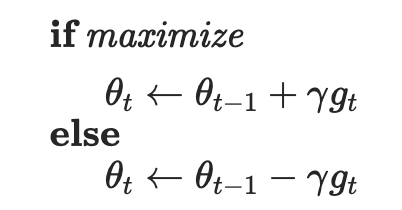
\includegraphics[scale=0.5]{figures/maximization.png}
        \end{figure}
        How do you think this change leads to the desired outcome (maximization vs minimization)? \\ 
        \solution{The gradient vector indicates the direction of steepest increase for a function. When minimizing, we move opposite to this direction by subtracting the gradient from our parameters, effectively descending toward lower values. When maximizing instead, we simply reverse this process by adding the gradient, which pushes our parameters in the direction of steepest increase. This sign flip transforms gradient descent into gradient ascent, allowing the same algorithm to handle both minimization problems and maximization problems without requiring separate implementations. The maximize parameter in PyTorch's SGD optimizer provides this flexibility with a boolean toggle.}
        \item The next set of parameters  {\tt momentum}, {\tt dampening}, {\tt weight\_decay}. What do you think the impact of these parameters are? Read the documentations and interpret their roles. \\
        \solution{Momentum, dampening, and weight decay in PyTorch's SGD optimizer each serve distinct but complementary roles in improving training. Momentum (typically 0.9) accumulates a velocity vector that helps navigate past local minima and flat regions by considering the history of gradients, similar to a rolling ball that maintains direction despite small obstacles. Dampening reduces the influence of the current gradient on this momentum term, stabilizing training when gradients are noisy. Weight decay implements L2 regularization by adding a penalty proportional to parameter magnitudes, preventing weights from growing too large and thus reducing overfitting. Together, these hyperparameters provide fine-tuned control over optimization dynamics, balancing between convergence speed, training stability, and model generalization.} 
    \end{enumerate}

    
    
    \item What are few benefits to using Fixed-Window-LM over $n$-grams language models? (limit your answer to less then 5 sentences). 
    \solution{Fixed-Window Language Models offer several advantages over traditional n-gram models. They maintain a consistent context window size regardless of the sequence length, which provides more stable performance across varying text spans. Their neural network architecture allows them to learn more nuanced semantic relationships and better generalize to unseen word combinations than the strict counting-based approach of n-grams. Fixed-Window models can more effectively handle data sparsity through distributed representations, eliminating the need for smoothing techniques required by n-gram models. Additionally, they typically require less storage space as they encode patterns in neural weights rather than storing explicit probability tables for all possible n-gram combinations.}

    \item When searching over hyperparameters, a typical recommendation is to do random search rather than a systematic grid search. 
    Why do you think that is the case? (less than 2 sentences). 
    % If searching among a large number of hyperparameters, you should try values in a grid rather than random values, so that you can carry out the search more systematically and not rely on chance. 
    \solution{Random search typically outperforms grid search because most machine learning models have only a few hyperparameters that significantly affect performance, and random search explores the high-importance dimensions more efficiently by testing more distinct values within those dimensions rather than wasting computational resources on exhaustive combinations.}
    \item Remember the normalization layer that we saw during the class. Here is the corresponding PyTorch page: \url{https://pytorch.org/docs/stable/generated/torch.nn.LayerNorm.html}. 
    In the normalization formula, why do we use epsilon $\epsilon$ in the denominator? \\ 
    \solution{The epsilon (ε) term is added to the denominator in the normalization formula to prevent division by zero. When the variance of the inputs is very small or zero, without epsilon, the normalization calculation would lead to numerical instability or undefined results. This small constant (typically set to values like 1e-5) ensures that the normalization operation remains stable even when dealing with inputs that have minimal variance, allowing the training process to continue smoothly without producing NaN values or causing the model to crash.}
    
\end{enumerate}

\section{Softmax Smackdown: Squishing the Competition}

\subsection{Softmax gradient}

You might remember in the midterm exam that we saw a neural network with a Softmax and a cross-entropy loss: 

$$ 
\hat{\textbf{y}} = \text{Softmax}(\textbf{h}),\; J = \text{CE}(\mathbf{y}, \hat{\mathbf{y}}), \hspace{1cm} \textbf{h}, \mathbf{y}, \hat{\mathbf{y}} \in \mathbb{R}^d.
$$
Basically here $\hat{\mathbf{y}}$ is a $d$-dimensional probability distribution over $d$ possible options (i.e. 
$\sum_i  \mathbf{y}_i = 1$ and $\forall i: \mathbf{y}_i \in [0, 1]$). 
$\mathbf{y}$ is a $d$-dimensional one-hot vector, i.e., all of these values are zeros except one that corresponds to the correct label. 

$$
\nabla_\mathbf{h} J = \hat{\mathbf{y}} - \mathbf{y}.
$$
Prove the above statement. 
In your proof, use the statement that you proved in HW3 about gradient of Softmax function: 
$\frac{ d \hat{\textbf{y}}_i }{ d \textbf{h}_j } = \hat{\textbf{y}}_i (\delta_{ij} - \hat{\textbf{y}}_j),$
        where $\delta_{ij}$ is the Kronecker delta function and $\hat{\textbf{y}}_i$ is the value in the $i$-th index of $\hat{\textbf{y}}$. \\ 
\solution{\begin{align*}
& J = -\sum_{i=1}^d y_i \log(\hat{y}_i) \\
& \text{Since $\mathbf{y}$ is one-hot at index $k$:} \quad J = -\log(\hat{y}_k) \\
\\
& \frac{\partial J}{\partial h_j} = -\frac{\partial \log(\hat{y}_k)}{\partial h_j} = -\frac{1}{\hat{y}_k}\frac{\partial \hat{y}_k}{\partial h_j} \\
& = -\frac{1}{\hat{y}_k}\hat{y}_k(\delta_{kj} - \hat{y}_j) = -(\delta_{kj} - \hat{y}_j) \\
\\
& \text{For $j = k$:} \quad \frac{\partial J}{\partial h_k} = -(1 - \hat{y}_k) = \hat{y}_k - 1 = \hat{y}_k - y_k \\
& \text{For $j \neq k$:} \quad \frac{\partial J}{\partial h_j} = -(-\hat{y}_j) = \hat{y}_j = \hat{y}_j - 0 = \hat{y}_j - y_j \\
\\
& \text{Therefore, for all $j$:} \quad \frac{\partial J}{\partial h_j} = \hat{y}_j - y_j \\
& \text{In vector form:} \quad \nabla_\mathbf{h} J = \hat{\mathbf{y}} - \mathbf{y}
\end{align*}}

\subsection{Softmax temperature}
Remember the softmax function, $\sigma(\mathbf{z})$? 
Here we will add a \emph{temperature} parameter $\tau \in \reals^+$ to this function: 
$$
    \text{Softmax: } \sigma(\mathbf{z}; \tau)_i = \frac{e^{z_i/ \tau}}{\sum_{j=1}^K e^{z_j/ \tau}} \ \ \text{ for } i = 1, \dotsc, K 
$$
Show the following: 
\begin{enumerate}
    \item In the limit as temperature goes to zero $\tau \rightarrow 0 $, softmax becomes the same as greedy action selection, {\tt argmax}.
    \solution{\begin{align*}
\text{Let } z_m = \max z_i \text{ be the maximum value in } z.\\
\\
\text{For any } i \text{ where } z_i < z_m:\\
\frac{e^{z_i/\tau}}{e^{z_m/\tau}} = e^{(z_i-z_m)/\tau} \to 0 \text{ as } \tau \to 0\\
\\
\text{Therefore:}\\
\sigma(z; \tau)_i \to 0 \text{ if } z_i < z_m\\
\sigma(z; \tau)_i \to 1 \text{ if } z_i = z_m\\
\\
\text{This is equivalent to the argmax operation.}
\end{align*}}
    \item In the limit as temperature goes to infinity $\tau \rightarrow +\infty$, softmax gives equiprobable selection among all actions. \\
    \solution{\begin{align*}
\text{As } \tau \to \infty, \frac{z_i}{\tau} \to 0 \text{ for all } i\\
\\
\text{Therefore:}\\
\lim_{\tau \to \infty} e^{z_i/\tau} = e^0 = 1 \text{ for all } i\\
\\
\lim_{\tau \to \infty} \sigma(z; \tau)_i = \frac{1}{\sum_{j=1}^K 1} = \frac{1}{K}\\
\\
\text{This gives equal probability } \frac{1}{K} \text{ to each action.}
\end{align*}}
\end{enumerate} 


\section{Backprop Through Residual Connections}  
    As you know, When neural networks become very deep (i.e. have many layers), they become difficult to train due to the vanishing gradient problem, as the gradient is back-propagated through many layers, repeated multiplication can make the gradient extremely small, so that performance plateaus or even degrades.
    An effective approach is to add skip connections that skip one or more layers. See the provided network. 

    \begin{figure}[ht]
        \centering
        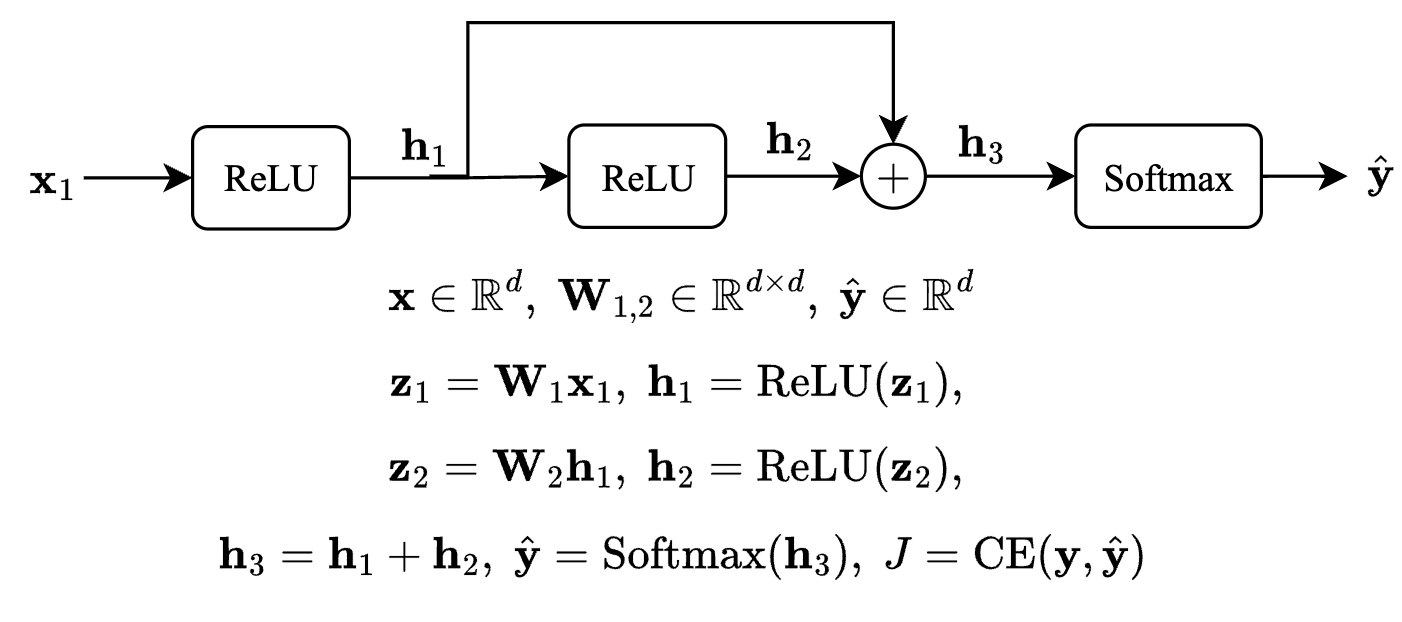
\includegraphics[scale=0.47]{figures/small-restnes.png}
    \end{figure}

\begin{enumerate}
    \item You have seen this in the quiz, but lets try again. Prove that: 
    $
    \frac{\partial }{\partial \textbf{z}_i} \text{ReLU}(\textbf{z}) = 1\{\textbf{z}_i > 0 \}
    $ where 
        $
    1\{x > 0 \} = \begin{cases}
    1 & \text{if} \; x> 0 \\ 
    0 &  \text{if} \; x \leq 0 \\ 
    \end{cases}
     $. More generally, 
     $\nabla_\textbf{z} \text{ReLU}(\textbf{z}) = \text{diag} \left( 1\{\textbf{z} > 0 \} \right)$ where $1\{.\}$ is applied per each dimension and $\text{diag}(.)$ turns a vector into a diagonal matrix.  

    \solution{ Definition of the ReLu Function:
$$
\text{ReLU}(z_i) = \max(0, z_i) = 
\begin{cases}
z_i & \text{if } z_i > 0 \\
0 & \text{if } z_i \leq 0
\end{cases}
$$ \\
Now, let's compute the derivative: \\
For $z_i > 0$:
$$\frac{\partial}{\partial z_i} \text{ReLU}(z_i) = \frac{\partial}{\partial z_i} z_i = 1$$ \\
For $z_i \leq 0$:
$$\frac{\partial}{\partial z_i} \text{ReLU}(z_i) = \frac{\partial}{\partial z_i} 0 = 0$$ \\
Therefore:
$$\frac{\partial}{\partial z_i} \text{ReLU}(z_i) = 
\begin{cases}
1 & \text{if } z_i > 0 \\
0 & \text{if } z_i \leq 0
\end{cases} = \mathbf{1}\{z_i > 0\}$$ \\
For a vector $z \in \mathbb{R}^n$, we have:
$$\text{ReLU}(z) = [\max(0, z_1), \max(0, z_2), \ldots, \max(0, z_n)]^T$$ \\
The gradient $\nabla_z \text{ReLU}(z)$ is the Jacobian matrix: \\
$$\nabla_z \text{ReLU}(z) = 
\begin{bmatrix}
\frac{\partial \text{ReLU}(z_1)}{\partial z_1} & \frac{\partial \text{ReLU}(z_1)}{\partial z_2} & \cdots & \frac{\partial \text{ReLU}(z_1)}{\partial z_n} \\
\frac{\partial \text{ReLU}(z_2)}{\partial z_1} & \frac{\partial \text{ReLU}(z_2)}{\partial z_2} & \cdots & \frac{\partial \text{ReLU}(z_2)}{\partial z_n} \\
\vdots & \vdots & \ddots & \vdots \\
\frac{\partial \text{ReLU}(z_n)}{\partial z_1} & \frac{\partial \text{ReLU}(z_n)}{\partial z_2} & \cdots & \frac{\partial \text{ReLU}(z_n)}{\partial z_n}
\end{bmatrix}$$ \\
Since $\text{ReLU}(z_i)$ only depends on $z_i$ and not on any other component of $z$, we have: \\
$$\frac{\partial \text{ReLU}(z_i)}{\partial z_j} = 
\begin{cases}
\frac{\partial \text{ReLU}(z_i)}{\partial z_i} & \text{if } i = j \\
0 & \text{if } i \neq j
\end{cases}$$ \\
From our scalar case proof, we know that $\frac{\partial \text{ReLU}(z_i)}{\partial z_i} = \mathbf{1}\{z_i > 0\}$. \\
Therefore, the Jacobian becomes: \\
$$\nabla_z \text{ReLU}(z) = 
\begin{bmatrix}
\mathbf{1}\{z_1 > 0\} & 0 & \cdots & 0 \\
0 & \mathbf{1}\{z_2 > 0\} & \cdots & 0 \\
\vdots & \vdots & \ddots & \vdots \\
0 & 0 & \cdots & \mathbf{1}\{z_n > 0\}
\end{bmatrix}$$ \\
This is precisely $\text{diag}(\mathbf{1}\{z > 0\})$, where $\mathbf{1}\{z > 0\}$ means the indicator function applied element-wise to each component of $z$.}

    \item As you see, a single variable ($\mathbf{h}_2$ in the example) feeds into two different layers of the network. Here we want to show that the two upstream signals stemming from this node are merged as summation  during Backprop. Specifically prove that: 
    $$
    \frac{\partial \mathbf{h}_3}{\partial \mathbf{h}_1 } = \textbf{I} + \frac{\partial \mathbf{h}_2}{\partial \mathbf{z}_2 } \frac{\partial \mathbf{z}_2}{\partial \mathbf{h}_1 } 
    $$

    \solution{First, we expand $h_3$ in terms of $h_1$ and $h_2$: \\
\begin{align*}
h_3 = h_1 + h_2
\end{align*} \\
Taking the derivative with respect to $h_1$: \\
\begin{align*}
\frac{\partial h_3}{\partial h_1} &= \frac{\partial h_1}{\partial h_1} + \frac{\partial h_2}{\partial h_1} \\
\end{align*} \\
We know that $\frac{\partial h_1}{\partial h_1} = I$ (identity matrix). \\
For the second term, we need to consider that $h_2 = f(z_2)$ and $z_2 = g(h_1)$ for some functions $f$ and $g$. 
By the chain rule: \\
\begin{align*}
\frac{\partial h_2}{\partial h_1} &= \frac{\partial h_2}{\partial z_2}\frac{\partial z_2}{\partial h_1}
\end{align*} \\
Therefore: \\
\begin{align*}
\frac{\partial h_3}{\partial h_1} &= I + \frac{\partial h_2}{\partial z_2}\frac{\partial z_2}{\partial h_1}
\end{align*} \\
This proves that the gradient from $h_3$ to $h_1$ is the sum of: \\
1. The direct gradient (identity matrix) from the skip connection
2. The gradient through the intermediate layer \\
This demonstrates why residual connections help with gradient flow - they allow gradients to flow back directly through the identity mapping, avoiding potential vanishing gradient problems.}


    \item 
    In the given neural network your task is to \textbf{compute the gradient 
    $\frac{\partial J}{ \partial \mathbf{x}}.$}    
    You are allowed (and highly encouraged) to use variables to represent intermediate gradients. 
    
\noindent    
\textbf{Hint 1:} Compute these gradients in order to build up your answer: 
$\frac{\partial \mathbf{J}}{\partial \textbf{h}_3}$,
$\frac{\partial \mathbf{J}}{\partial \textbf{h}_2}$,
$\frac{\partial \mathbf{J}}{\partial \textbf{z}_2}$,
$\frac{\partial \mathbf{J}}{\partial \textbf{h}_1}$,
$\frac{\partial \mathbf{J}}{\partial \textbf{z}_1}$,
$\frac{\partial \mathbf{J}}{\partial \textbf{x}}$. Show your work so we are able to give partial credit! 
    

\noindent
\textbf{Hint 2:} Recall that \emph{downstream = upstream * local}. 


\solution{\\ Step 1: $\frac{\partial J}{\partial h_3}$ \\
This is the gradient of the loss with respect to the final output. Let's denote this as:
\begin{align*}
\frac{\partial J}{\partial h_3} = \delta_{h_3}
\end{align*} \\
Step 2: $\frac{\partial J}{\partial h_2}$ \\
Using the chain rule:
\begin{align*}
\frac{\partial J}{\partial h_2} &= \frac{\partial J}{\partial h_3} \frac{\partial h_3}{\partial h_2} \\
&= \delta_{h_3} \cdot 1 \quad \text{(since $h_3 = h_1 + h_2$)} \\
&= \delta_{h_3}
\end{align*} \\
Step 3: $\frac{\partial J}{\partial z_2}$ \\
Applying the chain rule and using the ReLU derivative:
\begin{align*}
\frac{\partial J}{\partial z_2} &= \frac{\partial J}{\partial h_2} \frac{\partial h_2}{\partial z_2} \\
&= \delta_{h_3} \cdot \text{diag}(\mathbf{1}\{z_2 > 0\}) \\
&= \delta_{h_3} \odot \mathbf{1}\{z_2 > 0\} \\
&= \delta_{z_2}
\end{align*}
where $\odot$ represents element-wise multiplication. \\
Step 4: $\frac{\partial J}{\partial h_1}$ \\
$h_1$ affects $J$ through two paths: directly to $h_3$ and through $z_2$ to $h_2$ to $h_3$. 
\begin{align*}
\frac{\partial J}{\partial h_1} &= \frac{\partial J}{\partial h_3} \frac{\partial h_3}{\partial h_1} + \frac{\partial J}{\partial z_2} \frac{\partial z_2}{\partial h_1} \\
&= \delta_{h_3} \cdot 1 + \delta_{z_2} \cdot W_2 \\
&= \delta_{h_3} + \delta_{z_2} W_2 \\
&= \delta_{h_1}
\end{align*} \\
Step 5: $\frac{\partial J}{\partial z_1}$ \\
Similar to Step 3:
\begin{align*}
\frac{\partial J}{\partial z_1} &= \frac{\partial J}{\partial h_1} \frac{\partial h_1}{\partial z_1} \\
&= \delta_{h_1} \cdot \text{diag}(\mathbf{1}\{z_1 > 0\}) \\
&= \delta_{h_1} \odot \mathbf{1}\{z_1 > 0\} \\
&= \delta_{z_1}
\end{align*} \\
Step 6: $\frac{\partial J}{\partial x}$ \\
Finally:
\begin{align*}
\frac{\partial J}{\partial x} &= \frac{\partial J}{\partial z_1} \frac{\partial z_1}{\partial x} \\
&= \delta_{z_1} \cdot W_1 \\
&= \delta_{z_1} W_1
\end{align*} \\
Expanding this fully:
\begin{align*}
\frac{\partial J}{\partial x} &= \delta_{z_1} W_1 \\
&= (\delta_{h_1} \odot \mathbf{1}\{z_1 > 0\}) W_1 \\
&= ((\delta_{h_3} + \delta_{z_2} W_2) \odot \mathbf{1}\{z_1 > 0\}) W_1 \\
&= ((\delta_{h_3} + (\delta_{h_3} \odot \mathbf{1}\{z_2 > 0\}) W_2) \odot \mathbf{1}\{z_1 > 0\}) W_1
\end{align*} \\
This represents the complete gradient of $J$ with respect to $x$, computed by carefully tracking how the gradient flows backward through the network.}

    \item Based on your derivations, explain why residual connections help mitigate vanishing gradients. 
    \solution{Residual connections mitigate vanishing gradients by providing alternative pathways for gradient flow during backpropagation. As shown in our derivations, when we compute the gradient flowing back to a given layer, we get two components: a direct gradient from the residual connection, and a traditional gradient through the nonlinear transformation. The direct path ensures that at least some gradient flows back unimpeded, even if the traditional path suffers from vanishing gradients due to ReLU activations zeroing out signals or small weights diminishing them. This is evident in the formula $\frac{\partial J}{\partial h_1} = \delta_{h_3} + \delta_{z_2}W_2$, where $\delta_{h_3}$ represents the direct gradient that bypasses potential gradient-killing operations. Even if the second term approaches zero due to vanishing gradient issues, the first term still allows for learning. This gradient highway enables the training of much deeper networks than would otherwise be possible, as early layers can still receive meaningful learning signals regardless of network depth.}
\end{enumerate}





\clearpage
\section{Programming}
In this programming homework, we will
\begin{itemize}
    \item implement your own subword tokenizer.
    \item implement fixed-window MLP language models
\end{itemize}

\noindent \paragraph{Skeleton Code and Structure:}
The code base for this homework can be found at MyClasses Files under the \texttt{hw3} directory. Your task is to fill in the missing parts in the skeleton code, following the requirements, guidance, and tips provided in this pdf and the comments in the corresponding .py files.
The code base has the following structure:
\begin{itemize}
    \item \texttt{tokenization.py} implements the Byte-Pair Encoding algorithm for subword tokenization.
    \item \texttt{mlp\_lm.py} implements a fixed-window MLP-based language model on a subset of Wikipedia. 
    \item \texttt{main.py} provides the entry point to run your implementations in both \texttt{tokenizatiton.py} and \texttt{mlp\_lm.py}.
    \item \texttt{hw4.md} provides instructions on how to setup the environment and run each part of the homework in \texttt{main.py}
    
\end{itemize}

\noindent \todo{} ---
Your tasks include
1) generate plots and/or write short answers based on the results of running the code; 2) fill in the blanks in the skeleton to complete the code. We will explicitly mark these plotting, written answer, and filling-in-the-blank tasks as \todo{} in the following descriptions, as well as a \textcolor{blue}{\texttt{\textbf{\#~TODO}}} at the corresponding blank in the code. \\
\noindent \paragraph{Submission:} Your submission should contain two parts: 1) plots and short answers under the corresponding questions below; and 2) your completion of the skeleton code base, in a \texttt{.zip} file

\subsection{Tokenization Algorithms}
All NLP systems have \textit{at least} three main components that help machines understand natural language:
\begin{enumerate}
    \item Tokenization
    \item Embedding
    \item Model architectures
\end{enumerate}

Models like BERT, GPT-2 or GPT-3 all share the same components but with different architectures that distinguish one model from another.
We are going to focus on the first component of an NLP pipeline which is \textbf{tokenization}. An often overlooked concept but it is a field of research in itself. 
Though we have SOTA algorithms for tokenization it's always a good practice to understand the evolution trail. \\

\noindent Here's what we'll cover:
\begin{itemize}
    \item What is tokenization?
    \item Why do we need a tokenizer?
    \item Types of tokenization - Word, Character and Subword.
    \item Byte Pair Encoding Algorithm
    \item Other tokenization algorithms:
    \begin{itemize}
        \item Unigram Algorithm
        \item WordPiece - BERT transformer
        \item SentencePiece - End-to-End tokenizer system
    \end{itemize}
\end{itemize}

\subsubsection{What is Tokenization?}

Tokenization is the process of representing raw text in smaller units called tokens. These tokens can then be mapped with numbers to further feed to an NLP model.

\noindent Read and run the \texttt{full\_word\_tokenization\_demo} in \texttt{tokenization.py} for an overly simplified example of what a tokenizer does.

This is a very simple example where we just split a text string in to ``whole words'' on white spaces, and we have not considered grammar, punctuation, or compound words (like ``test'', ``test-ify'', ``test-ing'', etc.).

\paragraph{Problems with word tokenization:} \mbox{}\\
\begin{itemize}
    \item \textbf{Missing words in the training data}: With word tokens, your model won't recognize the variants of words that were not part of the data on which the model was trained. So, if your model has seen `foot` and `ball` in the training data but the final text has ``football'', the model won't be able to recognize the word and it will be treated with a ``<UNK>'' token. Similarly, punctuations pose another problem, ``let'' or ``let's'' will need individual tokens and it is an inefficient solution. This will \textbf{require a huge vocabulary} to make sure you've every variant of the word. Even if you add a \textbf{lemmatizer} to solve this problem, you're adding an extra step in your processing pipeline.
    \item \textbf{Not all languages use space for separating words}: For a language like Chinese, which doesn't use spaces for word separation, this tokenizer will fail.
\end{itemize}

\subsubsection{Character-based tokenization}
To resolve the problems associated with word-based tokenization, an alternative approach of character-by-character tokenization was tried. This solves the problem of missing words as now we are dealing with characters that can be encoded using ASCII or Unicode and it could generate embedding for any word now. 

Every character, be it space, apostrophes, or colons, can now be assigned a symbol to generate a sequence of vectors. But this approach had its cons. Character-based models will treat each character and will lead to longer sequences. For a 5-word long sentence, you may need to process 30 tokens instead of 5 word-tokens.

\subsubsection{Subword Tokenizaiton}
To address the earlier issues, we could think of breaking down the words based on a set of prefixes and suffixes. For example, we can build a system that can identify subwords like ``\#\#s'', ``\#\#ing'', ``\#\#ify'', ``un\#\#'' etc., where the position of double hash ``\#\#'' denotes prefix and suffixes. So, a word like ``unhappily'' is tokenized using subwords like ``un\#\#'', ``happ'', and ``\#\#ily''.

\textbf{BPE (Byte-Pair Encoding)} was originally a data compression algorithm that is used to find the best way to represent data by identifying the common byte pairs. It is now used in NLP to find the best representation of text using the least number of tokens.

Here's how it works:
\begin{enumerate}
    \item Add a ``</w>'' at the end of each word to identify the end of a word and then calculate the word frequency in the text.
    \item Split the word into characters and then calculate the character frequency.
    \item For a predefined number of iterations (set by you), count the frequency of the consecutive tokens and merge the most frequently occurring pairings.
    \item Keep iterating until you have reached the iteration limit or if you have reached the token limit.
\end{enumerate}
We will now go through this algorithm step by step.\\

\noindent Read the \texttt{get\_word\_freq} function in \texttt{tokenization.py} that implements the step 1 above to preprocess each word and count its frequency.\\

\noindent \todo{}: Read and complete the missing lines in the \texttt{get\_pairs} function in \texttt{tokenization.py} to implement the step 2 above. This function takes the word frequency record returned from \texttt{get\_word\_freq} as input, split the words into tokens (characters at this initial step), and counts token-pairs frequency.\\
\noindent \textbf{Hint}: follow the comments in the code for specific requirements.\\

\noindent Read the \texttt{get\_most\_frequent\_pair} and \texttt{merge\_byte\_pairs} functions in \texttt{tokenization.py} that implements the step 3 above, merge the top-1 frequent token-pairs in all the words.\\

In practise, after iterating over the input text for a desired number of times, we extract the resulting tokenization as our subword dictionary. For this purpose, we provide \texttt{get\_subword\_tokens} function in \texttt{tokenization.py}\\

\noindent With all these functions, we can now run one step of the BPE algorithm! \\

\noindent Read and run the \texttt{test\_one\_step\_bpe.py} in \texttt{main.py} to test the BPE algorithm for one step. A correct implementation of \texttt{get\_pairs} should pass all the tests.

\subsubsection{Complete the BPE Algorithm}
With the above implementations, we can complete all the steps of the BPE algorithm that iterates over the input corpus.\\

\noindent \todo{}: Read and complete the missing lines in the \texttt{exract\_bpe\_subwords} function in \texttt{tokenization.py} that implements the full BPE algorithm. Once you finished, run the \texttt{test\_bpe} function in \texttt{main.py}, a correct implementation of \texttt{exract\_bpe\_subwords} should pass all the tests.\\
\noindent \textbf{Hint}: follow the comments in the code and you can reuse the helper functions provided/you implemented above.\\

So as we iterate with each best pair, we merge (concatenating) the pair and you can see as we recalculate the frequency, the original character token frequency is reduced and the new paired token frequency pops up in the token dictionary.

\subsubsection{Running BPE on a subset of Wikipedia}
Now, let's run this algorithm on a larger scale. In particular, we will run on many Wikipedia paragraphs. As usual, let's use the Huggingface library to download the data (the \texttt{load\_bpe\_data} function).\\

\noindent \todo{}: Read and run the \texttt{bpe\_on\_wikitext} in \texttt{main.py} that iterates the BPE algorithm on a subset of Wikipedia, and interprets the final subwords extracted from the Wikipedia documents. In particular, identify examples of subwords that correspond to
\begin{enumerate}
    \item complete words
    \item part of a word
    \item non-English words(including other languages or common sequence special characters)
\end{enumerate}
Explain why these subwords have come about. (no more than 10 sentences)
\solution{Looking at the subwords extracted from the WikiText dataset, I can identify several patterns that demonstrate BPE's effectiveness as a tokenization algorithm. Complete words like "Hopkins</w>", "history</w>", and "government</w>" appear as tokens when they occur frequently enough to be merged as whole units. Partial words represent common morphemes that appear across many different words - examples include prefixes like "pro" and "com", suffixes like "tion" and "ment", and the common verb ending "ing". The algorithm also identified non-English characters and sequences, including diacritics, Greek letters, Arabic characters, East Asian characters, and special character sequences. These subwords emerged because BPE identified frequently occurring character sequences in the corpus, creating a vocabulary that balances between character-level tokenization (which would be too granular) and word-level tokenization (which would miss common subword patterns). This approach allows for efficient representation of text with fewer tokens, as the algorithm captures both standalone words and meaningful subword units across languages and special formatting found in the WikiText corpus.}

\subsubsection{Additonal Readings: Other Tokenization Algorithms}
\paragraph{WordPiece}\mbox{}\\
WordPiece is the subword tokenization algorithm used for \href{https://huggingface.co/docs/transformers/main/en/model_doc/bert}{BERT}, \href{https://huggingface.co/docs/transformers/main/en/model_doc/distilbert}{DistilBERT}, and \href{https://huggingface.co/docs/transformers/main/en/model_doc/electra}{Electra}. The algorithm was outlined in \citep{Schuster2012JapaneseAK} and is very similar to
BPE. WordPiece first initializes the vocabulary to include every character present in the training data and progressively learns a given number of merge rules. In contrast to BPE, WordPiece does not choose the most frequent symbol pair, but the one that maximizes the likelihood of the training data once added to the vocabulary.

So what does this mean exactly? Referring to the previous example, maximizing the likelihood of the training data is equivalent to finding the symbol pair, whose probability is divided by the probabilities of its first symbol followed by its second symbol is the greatest among all symbol pairs. E.g. ``u'', followed by ``g'' would have only been merged if the probability of ``ug'' divided by ``u'', ``g'' would have been greater than for any other symbol pair. Intuitively, WordPiece is slightly different from BPE in that it evaluates what it \textit{loses} by merging two symbols to ensure it's \textit{worth it}.

\paragraph{Unigram}\mbox{}\\
Unigram is a subword tokenization algorithm introduced in \citep{kudo2018subword}. In contrast to BPE or WordPiece, Unigram initializes its base vocabulary to a large number of symbols and progressively trims down each symbol to obtain a smaller vocabulary. The base vocabulary could for instance correspond to all pre-tokenized words and the most common substrings. Unigram is not used directly for any of the models in the transformers, but it's used in conjunction with SentencePiece(\autoref{paragraph:sentetncepiece}).

At each training step, the Unigram algorithm defines a loss (often defined as the log-likelihood) over the training data given the current vocabulary and a unigram language model. Then, for each symbol in the vocabulary, the algorithm computes how much the overall loss would increase if the symbol was to be removed from the vocabulary. Unigram then removes p (with p usually being 10\% or 20\%) percent of the symbols whose loss increase is the lowest, i.e. those symbols that least affect the overall loss over the training data. This process is repeated until the vocabulary has reached the desired size. The Unigram algorithm always keeps the base characters so that any word can be tokenized.

Because Unigram is not based on merge rules (in contrast to BPE and WordPiece), the algorithm has several ways of
tokenizing new text after training. As an example, if a trained Unigram tokenizer exhibits the vocabulary:
\\
\texttt{[``b'', ``g'', ``h'', ``n'', ``p'', ``s'', ``u'', ``ug'', ``un'', ``hug'']},

``hugs'' could be tokenized both as \texttt{[``hug'', ``s'']}, \texttt{[``h'', ``ug'', ``s'']} or \texttt{[``h'', ``u'', ``g'', ``s'']}. So which one to choose? Unigram saves the probability of each token in the training corpus on top of saving the vocabulary so that the probability of each possible tokenization can be computed after training. The algorithm simply picks the most likely tokenization in practice but also offers the possibility to sample a possible tokenization according to their probabilities.

Those probabilities are defined by the loss the tokenizer is trained on. Assuming that the training data consists of the words $x_{1}, \dots, x_{N}$ and that the set of all possible tokenizations for a word $x_{i}$ is defined as $S(x_{i})$, then the overall loss is defined as

$$\mathcal{L} = -\sum_{i=1}^{N} \log \left ( \sum_{x \in S(x_{i})} p(x) \right )$$

\paragraph{SentencePiece}\mbox{}\\ \label{paragraph:sentetncepiece}
All tokenization algorithms described so far have the same problem: It is assumed that the input text uses spaces to separate words. However, not all languages use spaces to separate words. One possible solution is to use language-specific pre-tokenizers, e.g. \href{https://huggingface.co/docs/transformers/main/en/model_doc/xlm}{XLM} uses a specific Chinese, Japanese, and Thai pre-tokenizer). To solve this problem more generally, \cite{kudorichardson2018sentencepiece} treats the input as a raw input stream, thus including the space in the set of characters to use. It then uses the BPE or unigram algorithm to construct the appropriate vocabulary.

The \href{https://huggingface.co/docs/transformers/main/en/model_doc/xlnet#transformers.XLNetTokenizer}{XLNetTokenizer} uses SentencePiece for example, which is also why in the example earlier the
``\textunderscore'' character was included in the vocabulary. Decoding with SentencePiece is very easy since all tokens can just be concatenated and ``\textunderscore'' is replaced by a space.

All transformer models in the library that use SentencePiece use it in combination with unigram. Examples of models using SentencePiece are \href{https://huggingface.co/docs/transformers/main/en/model_doc/albert}{ALBERT} \href{https://huggingface.co/docs/transformers/main/en/model_doc/xlnet}{XLNet},\href{https://huggingface.co/docs/transformers/main/en/model_doc/marian}{Marian}, and \href{https://huggingface.co/docs/transformers/main/en/model_doc/t5}{T5}.

\subsection{Fixed-Window MLP Language Models}
In the second part of the homework, we will build, train, and evaluate fixed-window MLP language models as we learned in class: given the context words in the fixed-size window on the left hand side, predict the next word continuation.

\begin{figure}[h]
    \centering
    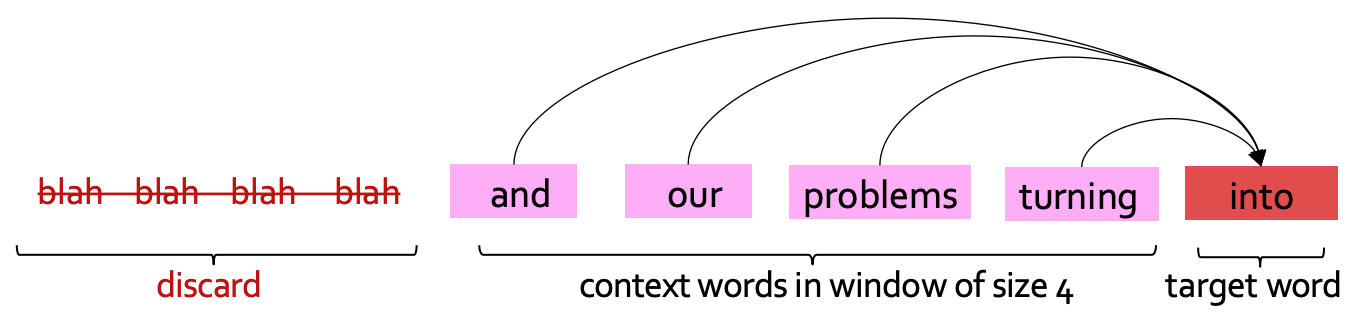
\includegraphics[width=0.45\textwidth]{figures/fixed_window_lm.png}
    \caption{Fixed-window LM}
\end{figure}

\subsubsection{Data Loading and Preprocessing}
We will be using the same \href{https://huggingface.co/datasets/wikitext}{WikiText} dataset we used for building n-gram LM in homework 2. We follow similar preprocessing steps to split paragraphs into sentences followed by tokenization (Now we have learned more about subword tokenization in class and the previous question!).\\

\noindent\todo{} read the \texttt{preprocess\_data} function in \texttt{ngram\_lm.py} and complete the missing lines to prepare input-output pairs for training fixed-window LMs.\\
\noindent \textbf{Hint}: follow the requirements in the code comments.

\subsubsection{Build our LM}
Let's now turn to building our model.
Here, we are following the footsteps of the neural probabilistic language model (NPLM) \citep{sun2021revisiting}, which is extending earlier studies such as \citet{bengio2003a}.   

\begin{figure}[h]
    \centering
    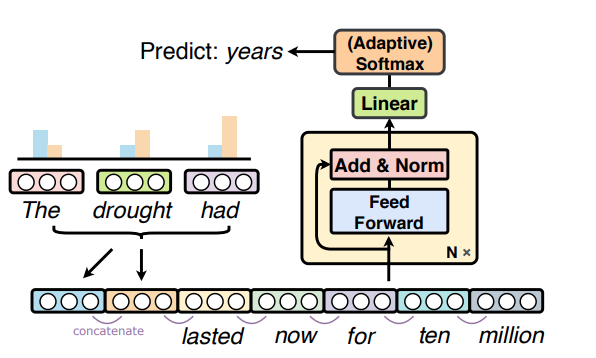
\includegraphics[width=0.45\textwidth]{figures/nplm.png}
    \caption{NPLM Architecture}
\end{figure}

We will follow a modular design for our implementation to make it more interpretable.
In particular, will implement 3 layers:
\begin{itemize}
    \item The \textbf{input layer} which loops up word embeddings, concatenates them, and transforms them into a hidden representation.
    \item The \textbf{middle layer} transforms the representation with a non-linearity.
    \item The \textbf{output layer} which transforms a hidden vector to a probability distribution over the words
\end{itemize}
Let's get to work!\\

\noindent\todo{}: read and complete the \texttt{forward} functions for the following classes
\begin{itemize}
    \item \texttt{NPLM\_first\_block}: input layer that embeds the input token ids into embedding vectors, concatenates the embeddings, applies linear transformation, layer normalization, and dropout 
    \item \texttt{NPLM\_block}: middle layers with linear transformation, tanh activation, residual connection, layer normalization, and dropout.
    \item \texttt{NPLM\_final\_block}: output layer that transforms hidden representation to log probability over the vocabulary with log softmax.
\end{itemize}
\textbf{Hint}: check out \href{https://pytorch.org/docs/stable/generated/torch.nn.LayerNorm.html}{nn.LayerNorm} and \href{https://pytorch.org/docs/stable/generated/torch.nn.Dropout.html}{nn.Dropout}, \href{https://pytorch.org/docs/stable/generated/torch.tanh.html}{torch.tanh} and \href{https://pytorch.org/docs/stable/generated/torch.nn.functional.log_softmax.html}{nn.functional.log\_softmax} for more details on these layers and operations. For embedding concatenation, you may find \href{https://pytorch.org/docs/stable/generated/torch.Tensor.view.html}{torch.Tensor.view} useful. Also, follow the step-by-step comments in the code for the requirements of the implementation.
\\\\
\noindent\todo{}: read and complete the \texttt{\_\_init\_\_} and \texttt{forward} functions for the \texttt{NPLM} class, which is the final model that stacks all the above layers.\\
\noindent \textbf{Hint}: remember to apply ReLU non-linear activation after each middle layer, details at \href{https://pytorch.org/docs/stable/generated/torch.nn.functional.relu.html}{nn.functional.relu}.
\subsubsection{Train and Evaluate the LM}
Now it's time to train and evaluate it! Like the previous homework, we will use cross-entropy loss between the predictions of our language model and actual words that appeared in our training data. Note that we applied log softmax to the final output of the LM, as described in homework to, we will use \href{https://pytorch.org/docs/stable/generated/torch.nn.NLLLoss.html#torch.nn.NLLLoss}{negative log-likelihood loss} as the training criterion to calculate the cross-entropy loss.

As introduced in the class, we will use \textbf{Perplexity} to evaluate our LM, as a measure of predictive quality of a language model. \\\\
\noindent \todo{} Read and complete the missing lines in \texttt{train} and \texttt{evaluate} functions in \texttt{mlp\_lm.py} to calculate the perplexity.\\
\noindent \textbf{Hint}: remember in the class we discussed the connection between perplexity and cross-entropy loss, and note that in our implementation we took natural logarithm instead of the base of 2.\\\\
Note we are using Adam \textbf{(Adaptive Moment Estimation)} \citep{kingma2015adam}, which is a popular optimization algorithm used in deep learning and machine learning. It is a stochastic gradient descent (SGD) optimization algorithm that is well suited for training deep neural networks. The algorithm has some internal estimates to dynamically adjust the learning rates for each parameter based on its past gradients, which can result in faster convergence and improved performance compared to traditional SGD.\\\\
\noindent \todo{} Once you finished all the implementations, run \texttt{load\_data\_mlp\_lm} and \texttt{single\_run\_mlp\_lm} in \texttt{main.py} to train and evaluate the model and paste the plots of loss and Perplexity here.\\
\noindent {\color{red}{your plots}}\\
% uncomment the following lines to add your plot
\begin{figure}[h] 
    \centering
    \subfloat[train and dev loss of the MLP LM]{
        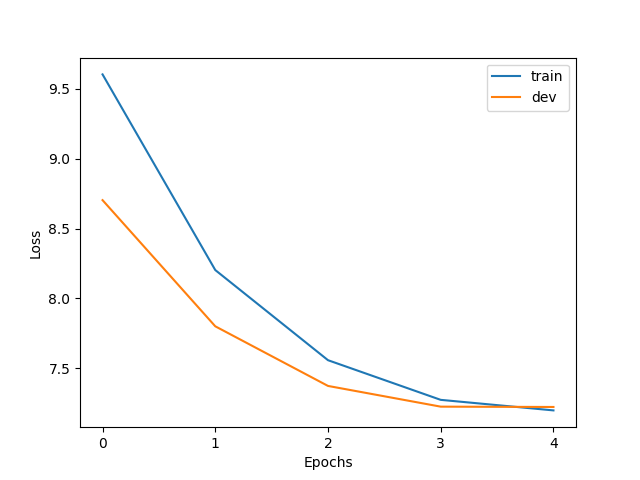
\includegraphics[width=0.45\textwidth]{figures/mlp_lm_loss.png}
        }
    \hfill
    \subfloat[train and dev ppl of the MLP LM]{
        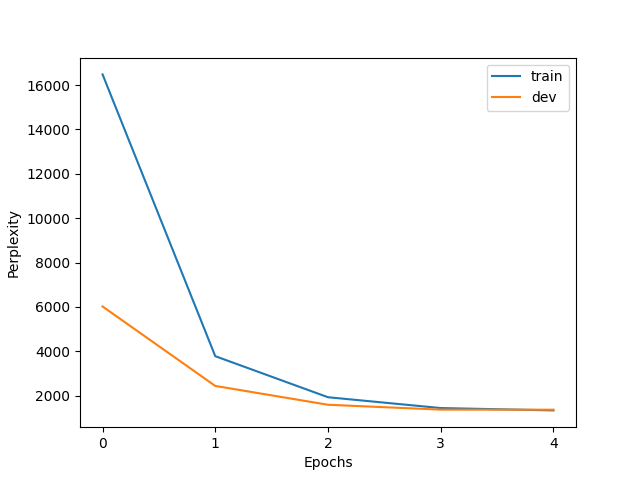
\includegraphics[width=0.45\textwidth]{figures/mlp_lm_ppl.png}
        }
    \caption{loss and ppl of the MLP LM}
\end{figure}

\subsubsection{Sample From a Pre-trained LM}
Note that compared with the original NPLM implementation, we reduce the model size by shrinking both the width and depth of our model, and we only use a small subset of the data. It is expected to take an hour or so to train the model on the CPU of your PC. Training the above LM with full size model and data might take hours to days. To save you time, we have trained a language model for you to play with. All you have to do is to download its weight parameters. Download the 
\href{https://livejohnshopkins-my.sharepoint.com/:u:/g/personal/dkhasha1_jh_edu/EW5N2dBb3ftAnQuannVNU_QBmmEn-VStlnVGWp5mRHdT-Q?e=NIChGd}{pre-trained weights} and copy it to your local directory under \texttt{/hw4/}.

Now that we have the model weight downloaded, we can instantiate a model with these parameters. This will work in two steps.
\begin{itemize}
    \item First we will need to create a new model (with potentially random weights).
    \item Then, we will copy the parameter values to the model using \href{https://pytorch.org/tutorials/beginner/saving_loading_models.html}{load\_state\_dict} function.
\end{itemize}
We then evaluate the loaded model on the dev set.
Now that we have loaded a pre-trained LM, how can we sample from it? We will implement two strategies, greedy decoding and top-p sampling \citep{holtzman2019curious} that we briefly discussed in homework 2.

For greedy, we select the most probable words (argmax).
\begin{figure}[h]
    \centering
    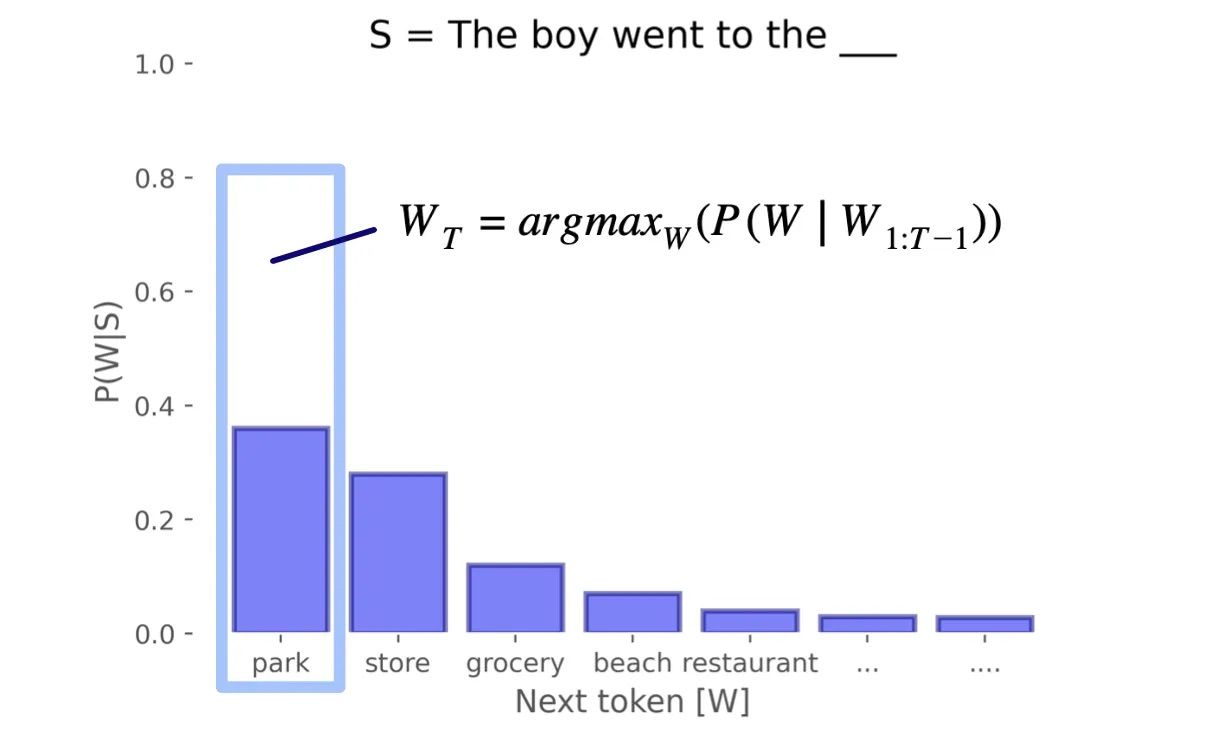
\includegraphics[width=0.45\textwidth]{figures/argmax_sampling.jpeg}
    \caption{Greedy Decoding}
\end{figure}

For top-p, we sample from the distribution proportional to word probabilities. Words with higher probabilities will be more likely to be sampled.
However, we also have an option of filtering the low-probability tokens, and instead retaining tokens that constitute texttt{top\_p} probability.
\begin{figure}[h]
    \centering
    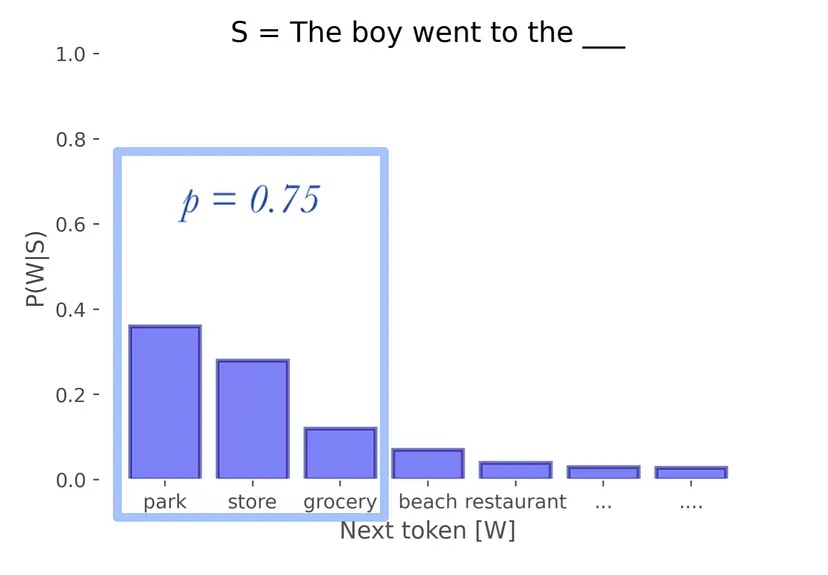
\includegraphics[width=0.45\textwidth]{figures/p_sampling.jpeg}
    \caption{Greedy Decoding}
\end{figure}

\noindent Read \texttt{generate\_text} and \texttt{sample\_from\_mlp\_lm} in \texttt{mlp\_lm.py} for more details about how to load the pre-trained model, evaluate on dev set and perform greedy/top-p sampling. You can learn more about top-p sampling implementation at \href{https://huggingface.co/docs/transformers/v4.37.2/en/internal/generation_utils#transformers.TopPLogitsWarper}{TopPLogitsWarper}.\\\\
\noindent \todo{} Run the \texttt{sample\_from\_trained\_mlp\_lm} in \texttt{main.py} to sample from the pre-trained LM, paste the completion to the prefix under different sampling strategies here, and describe in 2-3 sentences your findings.\\
\noindent \textbf{Hint}: compare the output of the above generations, which one is your favorite? Explain why this choice of sampling leads to better text generation.

\noindent \solution{Note: to generate the following output, some alterations were made to the provided code to prevent errors from inconsistent configurations and tensor shape mismatch. For example, embed dim: 128, hidden dim: 512, and num blocks: 2 \\ The configuration was updated to match the configuration for single run mlp lm. Also, if len(new input.shape) == 1:
new input = new input.unsqueeze(0). This was added to prevent tensor shape mismatch. \\ Here is the following output: \\
greedy: \qquad \qquad \qquad \,\,\, The best perks of living on the east..............................\\
top-p sampling (p=0.0): The best perks of living on the east..............................\\
top-p sampling (p=0.3): The best perks of living on the east of the of.. the, and of the. the.. of and and the of the of of of the.,. of.,\\
top-p sampling (p=1.0): The best perks of living on the east sense that are Valley. death by. her million @ - @ - @ of north, and to the all and. animated, of several.s\\
Looking at the generation results, we can observe that different sampling strategies significantly impact text quality. The greedy and p=0.0 sampling produces repetitive, unimaginative text that gets stuck in loops denoted by ..., while p=0.3 creates slightly more diverse but still incoherent output. I prefer the p=1.0 sampling because it generates the most varied and interesting text with actual content words like "Valley," "death," "million," and "animated." Although it's still not fully coherent, it shows more creativity and better approximates natural language by incorporating a wider vocabulary rather than repeating the same patterns.
}





\bibliographystyle{apalike}
\bibliography{ref}

\end{document}